% Load the kaobook class
\documentclass[
	ansiapaper,
	fontsize=11pt, % Base font size
	twoside=true, % Use different layouts for even and odd pages (in particular, if twoside=true, the margin column will be always on the outside)
	% open=any, % If twoside=true, uncomment this to force new chapters to start on any page, not only on right (odd) pages
	secnumdepth=1, % How deep to number headings. Defaults to 1 (sections)
]{kaobook}

\usepackage{sloth}


\begin{document}

%----------------------------------------------------------------------------------------
%	BOOK INFORMATION
%----------------------------------------------------------------------------------------

\titlehead{\centering
\includegraphics[width=.3\textwidth]{ugr_logo}}
\title[Mejoras en tratamiento de problemas de clasificación con modelos basados en autoencoders]{Mejoras en tratamiento de problemas de clasificación con modelos basados en autoencoders}
\subtitle{Tesis para la obtención del título de doctor por la Universidad de Granada\\Programa de doctorado en \textsc{Tecnologías de la Información y la Comunicación}}
\author[Francisco David Charte Luque]{Francisco David Charte Luque\\\texttt{<fdavidcl@ugr.es>}}
\department{Departamento de Ciencias de la Computación e Inteligencia Artificial}
\supervisor{Francisco Herrera Triguero\\Francisco Charte Ojeda}
\publicationplace{Granada}
\publicationdate{mayo de 2022}
\date{\underline{Directores de tesis}\\\textbf{Dr. D. Francisco Herrera}\\{\small Soft Computing y Sistemas de Información Inteligentes (Universidad de Granada)}\\\textbf{Dr. D. Francisco Charte}\\{\small Sistemas Inteligentes y Minería de Datos (Universidad de Jaén)}}
% \publishers{An Awesome Publisher}

%----------------------------------------------------------------------------------------

\frontmatter % Denotes the start of the pre-document content, uses roman numerals

%----------------------------------------------------------------------------------------
%	COPYRIGHT PAGE
%----------------------------------------------------------------------------------------

\makeatletter
\uppertitleback{\@title\\\@plainauthor} % Header

\lowertitleback{
	%\textbf{Disclaimer} \\
	%You can edit this page to suit your needs. For instance, here we have a no copyright statement, a colophon and some other information. This page is based on the corresponding page of Ken Arroyo Ohori's thesis, with minimal changes.
	
	%\medskip
	
	\textbf{Funding} \\
	This doctoral thesis was funded by the predoctoral program Formación del Profesorado Universitario (ref. FPU17/04069) from the Spanish Ministry of Universities.

	\medskip

	\textbf{Copyright} \\
	The published articles included in this document are printed with permission of their corresponding copyright holders:

	\begin{itemize}
		\item Articles~\ref{ch:paper1}, \ref{ch:paper2} and \ref{ch:paper5} are made available under the CC-BY-NC-ND 4.0 license according to Elsevier policy: \url{https://creativecommons.org/licenses/by-nc-nd/4.0}.
  		\item Copyright notice relative to Article~\ref{ch:paper3}: Reprinted by permission from Springer Nature: Springer Progress in Artificial Intelligence, A snapshot on nonstandard supervised learning problems: taxonomy, relationships, problem transformations and algorithm adaptations. David Charte, Francisco Charte, Salvador García, Francisco Herrera \textcopyright{} 2019.
    \item Copyright notice relative to Article~\ref{ch:paper6}: \textcopyright{} 2021 IEEE. Reprinted, with permission, from David Charte, Francisco Charte, Francisco Herrera. Reducing Data Complexity using Autoencoders with Class-informed Loss Functions. IEEE Transactions on Pattern Analysis and Machine Intelligence.
	\end{itemize}
	
	The rest of the contents of this book are released under the CC-BY-SA 4.0 copyright license. This allows you to share and modify it as long as the modifications are released under a similar license.

	To view a copy of the CC-BY-SA code, visit: \\\url{https://creativecommons.org/licenses/by-sa/4.0/}

	\medskip
	
	\textbf{Colophon} \\
	This document was typeset with the help of \href{https://sourceforge.net/projects/koma-script/}{\KOMAScript} and \href{https://www.latex-project.org/}{\LaTeX} using the \href{https://github.com/fmarotta/kaobook/}{kaobook} class.
	
	\medskip
	
	% \textbf{Publisher} \\
	% First printed in May 2019 by \@publishers
}
\makeatother

%----------------------------------------------------------------------------------------
%	DEDICATION
%----------------------------------------------------------------------------------------

\dedication{\itshape
	It's the questions we can't answer that teach us the most. They teach us how to think. If you give someone an answer, all they gain is a little fact. But give them a question and they'll look for their own answers. \\
	\flushright -- Patrick Rothfuss, The Wise Man's Fear\\\vspace{3em}
	Machines take me by surprise with great frequency. \\
	\flushright -- Alan Turing
}

%----------------------------------------------------------------------------------------
%	OUTPUT TITLE PAGE AND PREVIOUS
%----------------------------------------------------------------------------------------

% Note that \maketitle outputs the pages before here
\makeouterpage
\maketitle

\clearpage
~
\vspace{5cm}

El doctorando \textbf{Francisco David Charte Luque} y los directores de la tesis \textbf{Dr. D. Francisco Herrera Triguero} y \textbf{Dr. D. Francisco Charte Ojeda}\\Garantizamos, al firmar esta tesis doctoral, que el trabajo ha sido realizado por el doctorando bajo la dirección de los directores de la tesis y, hasta donde nuestro conocimiento alcanza, en la realización del trabajo se han respetado los derechos de otros autores a ser citados, cuando se han utilizado sus resultados o publicaciones.

\vspace{1cm}
The doctoral candidate \textbf{Francisco David Charte Luque} and the thesis supervisors \textbf{Dr. D. Francisco Herrera Triguero} y \textbf{Dr. D. Francisco Charte Ojeda}\\Gaurantee, by signing this doctoral thesis, that the work has been done by the doctoral candidate under the direction of the thesis supervisors and, as far as our knowledge reaches, in the performance of the work, the rights of other authors to be cited (when their results or publications have been used) have been respected.
\vspace{1cm}

\begin{center}
    Granada, 19 de mayo de 2022\\\vspace{1em}
    Doctorando\\
    \vspace{3cm}
    Directores de la tesis
\end{center}
\clearpage

\pagestyle{pagenum.scrheadings}

%----------------------------------------------------------------------------------------
%	PREFACE
%----------------------------------------------------------------------------------------
\pagelayout{margin}
\chapter*{Acknowledgments}


I hope the reader appreciates the hard work that has ultimately produced this thesis, which is the result of the direct and indirect effort of many people. 

First and foremost, I am infinitely grateful for the opportunities, guidance, help and trust my supervisors have offered me. I have been extremely lucky to have such passionate, knowledgeable and caring people directing this work. These four years have allowed me to be creative, to learn much more and to go beyond even what I expected. Thank you, dad. Thank you, Paco.

Learning is one of my passions. I am thankful for all the good teachers I have had, they are the motivation that students need to strive for the best. I want to take a moment to thank and remember two of them who sadly are no longer with us. With Manuel Arroquia I learned not to accept something as truth without finding a reasoning. Julio Ortega showed me that there is joy in teaching and caring about your students. The curiosity you inspired in your students and the aspiration for excellence you inspired in your colleagues live on.

Big thanks to my friends in the SCI2S group and at the CITIC for making these years fun, making me see things from other perspectives and being there to support each other.

It is fairly uncommon that one of your supervisors also happens to be your father. Because of this, the rest of my family had to bear with many boring conversations at home when work topics inevitably came up. Still, they have always been there to share a good time with us. Mom, Alex, thank you for your endless patience and support.

Finally, I have to express my gratitude to the person who has always been next to me during these four years, who has lifted my spirits more times than I could count and has shown me nothing but love. Thank you from the bottom of my heart, Esperanza.

This work is a reality thanks to all of you.

\pagelayout{wide}
% \pagelayout{margin}%
\chapter*{Abstract}

\begin{center}
\textbf{Improvements in treatment of classification problems with autoencoder-based models}
\end{center}

The present doctoral thesis tackles the study and application of a specific tool from the data science field, autoencoders, which are artificial neural networks able to transform the variable space of a dataset according to a certain selected criterion. Manipulating and transforming variables is a crucial task in data mining, since it can largely determine the complexity of a data analysis problem and, as a result, affect the behavior of learning methods which are used to extract useful knowledge. Moreover, the recent surge in data collection and processing for all kinds of purposes causes these tasks to be less and less feasible to be performed by hand, so there is a need of automatic methods to solve them.

Autoencoders are models that belong to the field of representation learning, and can be much more flexible and adaptable than other, more classical methods such as principal component analysis. This versatility has been studied via a thorough analysis of their inner workings and the different varieties of models than can be created based on their essential components. As a complement, a new software tool has been developed to provide easy access to these models and eliminate an important existing knowledge barrier which could prevent their use.

An extensive search has been conducted in the literature for problem typologies whose difficulty is related to the data representation, so as to open the possibility for autoencoder-based solutions. Datasets can present several issues: those linked to the very structure of the data points, like the use of several objects to describe a sole instance; those relative to the complexity of categorized data, or tasks that do not provide additional information and must be solved by means of feature analysis.

With the aim of creating a novel contribution in the field of autoencoders, three new models have been developed to tackle the problem of complexity in categorized data. They are able to simplify the borders between categories in order for a classification method to improve its performance.

In summary, the main contributions of this thesis are as follows:

\begin{itemize}
    \item A \textbf{theoretical analysis and taxonomy} of the main autoencoder variants present in the literature, composing a guide to ease their selection and use.
    \item A complete \textbf{software package} which automatizes a great part of the implementation work for autoencoders and simplifies its use to a level similar to other feature extraction methods.
    \item A \textbf{synthesis and organization} work of the peculiarities that supervised learning problems can present when data points are represented in a nonstandard fashion.
    \item A \textbf{demonstration of the diverse applications} of autoencoder-based models, identifying and exposing several strategies to solve unsupervised problems by means of variable transformations.
    \item Three new models, \textbf{Scorer, Skaler and Slicer}, focused on data complexity reduction in classification problems.
\end{itemize}

This document introduces all global concepts needed to understand the published articles and provides a theoretical vision of the representation learning problem and of the deep learning tool set, which includes the main object of study. In addition, it explains the techniques that help put into practice these models and how they execute on computation infrastructures. Next, the material published throughout the doctoral period is introduced and five articles published in renowned journals are reproduced. Finally, these and other activities carried out are summarized and the lines of work that would continue the achieved advancements are presented.

\pagelayout{wide}%
% \pagelayout{margin}%
\chapter*{Resumen}

\begin{center}
\textbf{Mejoras en tratamiento de problemas de clasificación con modelos basados en autoencoders}
\end{center}

La presente tesis doctoral aborda el estudio y aplicación de una herramienta particular del ámbito de la ciencia de datos, los \textit{autoencoders}, que son redes neuronales artificiales capaces de transformar el espacio de variables de un conjunto de datos según un criterio escogido. La manipulación y transformación de variables es una tarea crucial en minería de datos, puesto que puede determinar en gran medida lo complejo que resulte un problema de análisis de datos y, por tanto, afectar al comportamiento de los métodos de aprendizaje con los que se pretende extraer conocimiento útil. Además, el reciente incremento en recolección y procesamiento de datos para todo tipo de propósitos propicia que cada vez menos tareas de transformación se puedan realizar manualmente, por lo que son necesarios métodos automáticos que las resuelvan. 

Los \textit{autoencoders} son modelos que se encuadran en el campo del aprendizaje de representaciones, y resultan mucho más flexibles y adaptables que otros métodos más clásicos como el análisis de componentes principales. Para estudiar esta versatilidad, se ha realizado un análisis pormenorizado de su funcionamiento y de las diferentes variedades de modelos que se pueden crear fundamentándose en sus componentes básicos. Como complemento, se ha construido una herramienta software que proporciona fácil acceso a estos modelos y elimina una importante barrera de conocimiento existente a la hora de utilizar los \textit{autoencoders}.

Asimismo, se ha llevado a cabo una extensa búsqueda en la literatura de tipologías de problemas cuya dificultad esté relacionada con la representación de los datos, de forma que se pueda plantear una solución basada en \textit{autoencoders}. Se han identificado varias clases de conflictos que pueden presentar los conjuntos de datos: los que residen en la propia estructura de los datos como, por ejemplo, el uso de varios objetos para representar una sola instancia; los relacionados con la complejidad de los propios datos cuando están categorizados, o tareas que no aportan información adicional y han de resolverse por medio del análisis de las características.

Con el objetivo de aportar una contribución novedosa al campo de los \textit{autoencoders}, se han desarrollado tres modelos que abordan el problema de la complejidad de los datos categorizados, siendo capaces de simplificar las fronteras entre las categorías de forma que un método de clasificación mejore su rendimiento.

En resumen, las principales contribuciones de la tesis son las siguientes:

\begin{itemize}
    \item Un \textbf{análisis teórico y taxonomía} de las principales variantes de \textit{autoencoders} presentes en la literatura, componiendo una guía para facilitar la selección y el uso de las mismas.
    \item Un completo \textbf{paquete software} que automatiza gran parte del trabajo de implementación de \textit{autoencoders} y acerca su uso a un nivel comparable al de otros métodos de extracción de características más simples.
    \item Un trabajo de \textbf{organización y síntesis} de las particularidades que pueden presentar los problemas de aprendizaje supervisado cuando los datos están representados de formas no estándares.
    \item Una \textbf{demostración de las diversas aplicaciones} de los modelos basados en \textit{autoencoders}, identificando y exponiendo distintas estrategias para resolver problemas no supervisados mediante manipulación de las variables.
    \item Tres nuevos modelos, \textbf{Scorer, Skaler y Slicer}, enfocados a la reducción de la complejidad de datos en problemas de clasificación.
\end{itemize}

El presente documento introduce todos los conceptos globales necesarios para entender los artículos publicados y aporta una visión teórica de la problemática del aprendizaje de representaciones y del conjunto de herramientas de aprendizaje profundo, dentro del cual se enmarca el objeto principal de estudio. Además, se explican las técnicas que ayudan a llevar a la práctica estos modelos y cómo se ejecutan sobre las infraestructuras de computación. Posteriormente se introduce el material publicado a lo largo del periodo doctoral y se reproducen cinco artículos publicados en revistas científicas de notable reputación. Finalmente se resumen estas y otras actividades llevadas a cabo, y se presentan las líneas de trabajo que continuarían con los avances ya realizados.



\pagelayout{wide}%

%----------------------------------------------------------------------------------------
%	TABLE OF CONTENTS & LIST OF FIGURES/TABLES
%----------------------------------------------------------------------------------------

\begingroup % Local scope for the following commands

% Define the style for the TOC, LOF, and LOT
%\setstretch{1} % Uncomment to modify line spacing in the ToC
%\hypersetup{linkcolor=blue} % Uncomment to set the colour of links in the ToC
\setlength{\textheight}{230\vscale} % Manually adjust the height of the ToC pages

% Turn on compatibility mode for the etoc package
\etocstandarddisplaystyle % "toc display" as if etoc was not loaded
\etocstandardlines % "toc lines as if etoc was not loaded

\tableofcontents % Output the table of contents
% \clearpage
\listoffigures % Output the list of figures

% Comment both of the following lines to have the LOF and the LOT on different pages
% \let\cleardoublepage\bigskip
% \let\clearpage\bigskip

\listoftables % Output the list of tables

\endgroup


%----------------------------------------------------------------------------------------
%	MAIN BODY
%----------------------------------------------------------------------------------------

\mainmatter % Denotes the start of the main document content, resets page numbering and uses arabic numbers
\setchapterstyle{kao} % Choose the default chapter heading style

\makepart{Fundaments}
\includechapter{intro} 
\includechapter{theory}

\includechapter{practical}

\makepart{Published articles}

\includechapter{summary}

\setcounter{margintocdepth}{\sectiontocdepth}
\includearticle{01-autoencoder-review}
\setListingsForR
\includearticle{02-ruta}
\includearticle{03-nonstandard}
\includearticle{05-case-studies} 
\includearticle{06-reducing}
\setcounter{margintocdepth}{\subsectiontocdepth}

% \includearticle{04-showcase}
% \includearticle{07-slicer} 
 
\makepart{Final remarks}

\includechapter{conclusions}
% \setchapterpreamble[u]{\margintoc}
\chapter{Conclusions}
\label{ch:conclusions}

This chapter aims to summarize the outcomes of this thesis, highlight the most relevant achievements, list the related published material and outline some lines of work that will be pursued next.

\section{Achieved objectives}

Before detailing specific results, this section explains how the different objectives posed at the beginning of the thesis have been tackled and completed.

\subsection{Didactic resources for learning about autoencoders}

Autoencoders are conceptually very different from traditional feature extractors. Unlike these, autoencoders are based on a neural network framework and this allows for a high level of customization and adjustments for each task. However, this availability of diverse options when building an autoencoder makes it less accessible to inexperienced practitioners. This is a barrier that was identified at; the start of our research work and, as a result, became an issue we wanted to address.

Our first goal, taking advantage of the usual literature review, was to produce a guide on autoencoders for machine learning users assuming no prior knowledge about neural networks or these models in particular. This guide should cover all the basics in order to be able to grasp what autoencoders compute, how they are trained, how they compare to other feature learners and what options a user may be presented with when choosing to apply this model to their data.

The result was an extensive article (reproduced as \autoref{paper1}) that explained every fundamental aspect about these models, as well as provided enough detail about the main variants to be able to select an appropriate one for any given purpose. One key contribution of this work was \autoref{p1Sec.HowToChoose}, which attempts to provide advice on which options to choose depending on the problem at hand.

\subsection{Software tool for easy access to autoencoders}

One of the first obstacles that programmers may come across when working with feature learning tools is that autoencoders are much harder to set up and train than other alternatives like PCA or even complex manifold learning algorithms such as LLE or Isomap, which come already implemented in libraries and can be applied with a simple function call.

The main software-related outcome of this thesis has been the R package Ruta, a library which includes the most relevant autoencoder variants and provides easy-to-use functionalities for beginners, as well as more flexible and detailed options for more experienced users. This software is published at CRAN, a software repository for the R language with strict quality controls.

The Ruta package has totaled more than 15000 downloads just on the official RStudio CRAN mirror, averaging more than 10 downloads per day since its launch. Figure~\ref{fig:rutadl} shows daily downloads of the library according to the RStudio CRAN logs.

\begin{figure*}[htbp]
    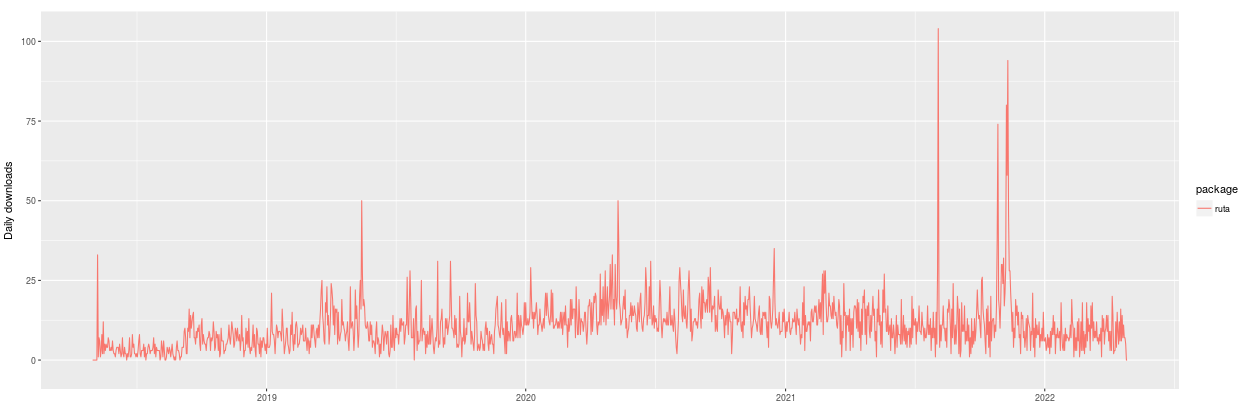
\includegraphics{rutadownloads}
    \caption{\label{fig:rutadl}Per-day downloads of the Ruta package from the RStudio CRAN mirror.}
\end{figure*}

\subsection{Development of new autoencoder losses for class separability}

After a more general focus on the state of the art, it was important to create new solutions based on what had been learned. These solutions should be applicable as widely as possible and tackle real problems from a novel perspective, leveraging the flexibility of autoencoders.

In order to contribute to the specific field of autoencoders, our aim was to improve on one of the main uses that these models can have, the extraction of better features for classification methods. Instead on relying on the intended classifiers themselves to optimize the quality of the features, like a deep neural network would operate, we opted to choose metrics that inform about the ability of dataset variables to separate different classes. This way, the model is not necessarily focused on the variables that are more relevant to allow a neural network classify, but those that help separate classes in general, which can in turn be useful for various classifiers.

The extensive experimentation showed that, out of the three methods considered, the LSSVM-inspired loss worked best and provided significant improvement in classification performance with respect to other feature learners.

\subsection{Application of newly developed models}

The previous model proposal would be more valuable if useful applications of it were deployed. For a first use, we chose a dataset that was imposing notable levels of difficulty for classifiers to model adequately, the COVIDGR dataset of chest X-ray imaging for COVID-19 detection. This is, as well, an area where a solution involving a simple, interpretable classifier would appeal more to the experts than a black-box model like a neural network.

The results revealed a promising line of work, as several of the selected classifiers improved their performance when learning from the features extracted by the proposed model with respect to the original features.

\section{Summary of publications}

This section holds a relation of all public results of the thesis, including the publications that have been reproduced from \autoref{ch:paper1} to \autoref{ch:paper6}, the related software packages and repositories that allow to replicate experimental results, as well as publications arising from collaborations with colleagues and other projects.

\subsection{Publications associated to the thesis}

Following are the publications in JCR journals and international conferences associated to the present thesis.

\subsubsection{Publications in JCR journals}

Next are the five articles published in journals listed in JCR which are directly linked to the thesis. Four of them are published in Q1 journals, including an article in IEEE TPAMI which is the highest ranking journal in the area of Computer Science-Artificial Intelligence according to JCR. The remaining article, published in Progress in Artificial Intelligence, is listed as Q4 in the ESCI (Emerging Sources Citation Index) ranking.

\begin{itemize}
    \item Charte, D., Charte, F., García, S., del Jesus, M. J., \& Herrera, F. (2018). A practical tutorial on autoencoders for nonlinear feature fusion: Taxonomy, models, software and guidelines. Information Fusion, 44, 78-96.
    \item Charte, D., Charte, F., García, S., \& Herrera, F. (2019). A snapshot on nonstandard supervised learning problems: taxonomy, relationships, problem transformations and algorithm adaptations. Progress in Artificial Intelligence, 8(1), 1-14.
    \item Charte, D., Herrera, F., \& Charte, F. (2019). Ruta: Implementations of neural autoencoders in R. Knowledge-Based Systems, 174, 4-8.
    \item Charte, D., Charte, F., del Jesus, M. J., \& Herrera, F. (2020). An analysis on the use of autoencoders for representation learning: Fundamentals, learning task case studies, explainability and challenges. Neurocomputing, 404, 93-107.
    \item Charte, D., Charte, F., \& Herrera, F. (2021). Reducing Data Complexity using Autoencoders with Class-informed Loss Functions. IEEE Transactions on Pattern Analysis and Machine Intelligence.
\end{itemize}

\subsubsection{Communications in international conferences}

Two works were presented in international conferences:

\begin{itemize}
    \item Charte, D., Charte, F., del Jesus, M. J., \& Herrera, F. (2019, June). A Showcase of the Use of Autoencoders in Feature Learning Applications. In International Work-Conference on the Interplay Between Natural and Artificial Computation (pp. 412-421). Springer, Cham.
    \item Charte, D., Sevillano-García, I., Lucena-González, M. J., Martín-Rodríguez, J. L., Charte, F., \& Herrera, F. (2021, September). Slicer: Feature Learning for Class Separability with Least-Squares Support Vector Machine Loss and COVID-19 Chest X-Ray Case Study. In International Conference on Hybrid Artificial Intelligence Systems (pp. 305-315). Springer, Cham.
\end{itemize}


\subsection{Published software}

Most of the developed software to perform experimentations has been made available in the popular code repository GitHub for its use to replicate and extend them. Additionally, some of these packages conveniently allow users to apply the models to other datasets, more specifically, Ruta and the autoencoders for complexity reduction including the convolutional version of Slicer.

\begin{itemize}
    \item Ruta, software for unsupervised deep architectures (associated to \autoref{ch:paper2}). Homepage: \href{https://ruta.software/}{ruta.software}. Source code: \href{https://github.com/fdavidcl/ruta}{github.com/fdavidcl/ruta}.
    \item autoencoder-showcase (associated to \autoref{ch:paper4}). Homepage/source code: \href{https://github.com/ari-dasci/S-autoencoder-showcase}{github.com/ari-dasci/S-autoencoder-showcase}.
    \item ae-case-studies (associated to \autoref{ch:paper5}). Homepage/source code: \href{https://github.com/fdavidcl/ae-case-studies}{github.com/fdavidcl/ae-case-studies}.
    \item Reducing complexity (associated to \autoref{ch:paper6}). Homepage: \href{https://ari-dasci.github.io/S-reducing-complexity/}{ari-dasci.github.io/S-reducing-complexity}. Source code: \href{https://github.com/ari-dasci/S-reducing-complexity}{github.com/ari-dasci/S-reducing-complexity}.
    \item Convolutional Slicer (associated to \autoref{ch:paper7}). Homepage/source code: \href{https://github.com/fdavidcl/slicer-conv}{github.com/fdavidcl/slicer-conv}.
\end{itemize}

\subsection{Collaborations and other related results}

This section is dedicated to works published during the thesis period where the doctoral candidate participated, as well as talks and dissemination material around the topic of the present thesis.

\subsubsection{Articles published in collaboration with other researchers with tangential topics to the current thesis}

The following are five JCR articles whose topics interleave with the present thesis but are not core to the main objectives. 

\begin{itemize}
    \item Charte, F., Rivera, A. J., \textbf{Charte, D.}, del Jesus, M. J., \& Herrera, F. (2018). Tips, guidelines and tools for managing multi-label datasets: The mldr.datasets R package and the Cometa data repository. Neurocomputing, 289, 68-85.
    \item Górriz, J. M., Ramírez, J., Ortíz, A., Martinez-Murcia, F. J., Segovia, F., Suckling, J., \dots \textbf{Charte, D.}, \dots \& Ferrández, J. M. (2020). Artificial intelligence within the interplay between natural and artificial computation: Advances in data science, trends and applications. Neurocomputing, 410, 237-270.
    \item Tabik, S., Gómez-Ríos, A., Martín-Rodríguez, J. L., Sevillano-García, I., Rey-Area, M., \textbf{Charte, D.}, \dots \& Herrera, F. (2020). COVIDGR dataset and COVID-SDNet methodology for predicting COVID-19 based on chest X-ray images. IEEE Journal of biomedical and health informatics, 24(12), 3595-3605.
    \item Pascual-Triana, J. D., \textbf{Charte, D.}, Andrés Arroyo, M., Fernández, A., \& Herrera, F. (2021). Revisiting data complexity metrics based on morphology for overlap and imbalance: snapshot, new overlap number of balls metrics and singular problems prospect. Knowledge and Information Systems, 63(7), 1961-1989.
    \item Luengo, J., Moreno, R., Sevillano, I., \textbf{Charte, D.}, Peláez-Vegas, A., Fernández-Moreno, M., \dots \& Herrera, F. (2022). A tutorial on the segmentation of metallographic images: Taxonomy, new MetalDAM dataset, deep learning-based ensemble model, experimental analysis and challenges. Information Fusion, 78, 232-253.
\end{itemize}

\subsubsection{Other conferences and talks}

The following talks and works were presented in national-level conferences and other events:

\begin{itemize}
    \item Charte, D., Charte, F., Herrera, F. (2017). Unsupervised Deep Learning in R with Ruta. Poster presented at \textit{IX Jornadas de Usuarios de R} in Granada.
    \item Charte, D., Charte, F., García, S., del Jesus, M.J., Herrera, F. (2018). Keywork "A practical tutorial on autoencoders for nonlinear feature fusion" presented at \textit{XVIII Conferencia de la Asociación Española para la Inteligencia Artificial (CAEPIA)} in Granada.
    \item Charte, D. (2019). Aplicaciones prácticas de las redes neuronales no supervisadas. Talk presented at \textit{esLibre 2019} within track "Informática y matemáticas", in Granada.
    \item Charte, D. (2020). Autoencoders: An Overview and Applications. Talk presented at \textit{IAA-CSIC Severo Ochoa School on Machine Learning, Big Data, and Deep Learning in Astronomy (SOMACHINE 2020)}.
\end{itemize}

\subsubsection{Educational/training material}

During the course of the thesis, a textbook on machine learning and data science has been published for use as training material, as well as a 5-video course on linear algebra and dimensionality reduction, including autoencoder networks:

\begin{itemize}
    \item Charte, Francisco \& Charte, David (2021). Machine Learning y Ciencia de Datos con Python y R. Krasis Consulting. ISBN: 978-8494582257.
    \item Math-ML Course, Module 2: Linear algebra and dimensionality reduction. Published in collaboration with the Andalusian Research Institute in Data Science and Computational Intelligence (DaSCI). Video playlist: \href{https://www.youtube.com/playlist?list=PL88MWrW4s4nf-Bc3hccxt3Att8TSS-LBn}{youtube.com/ playlist?list=PL88MWrW4s4nf-Bc3hccxt3Att8TSS-LBn}.
\end{itemize}

\subsubsection{Projects with public and private entities}

\begin{itemize}
    \item Our research group has participated in several state-funded projects which involve deep learning as one of their main lines of work. Their funding allowed the group to build the necessary infrastructure to quickly develop and test models with large amounts of data.
    \item The candidate has collaborated with the Repsol statistics department in optimization of refinery processes. No research outputs are available due to industrial secrecy requirements.
    \item The candidate has participated in a two-year collaboration with the metallurgic company ArcelorMittal, on the topic of semantic segmentation of metallographic iamges with encoder-decoder deep neural networks. A result of this project was the article ``A tutorial on the segmentation of metallographic images: Taxonomy, new MetalDAM dataset, deep learning-based ensemble model, experimental analysis and challenges'' co-written by the UGR and ArcelorMittal teams.
    \item A collaboration was also established with the Hospital Universitario San Cecilio in Granada, during which the candidate looked into capsule networks and convolutional networks attempting to solve the problem of detecting the presence of COVID-19-induced lung affection. The results of this study were published in the article ``COVIDGR dataset and COVID-SDNet methodology for predicting COVID-19 based on chest X-ray images''.
\end{itemize}

% \setchapterpreamble[u]{\margintoc}
\section{Future lines of work}
% \label{ch:future}

The developed work has shown to be very promising and opens several possible routes to continue researching. 

\subsection{Label separability in multi-label data}

\subsection{Promoting other behavior in learned representations}

\subsection{Synthetic instance generation for label resampling}

 

%----------------------------------------------------------------------------------------

\backmatter % Denotes the end of the main document content
\setchapterstyle{plain} % Output plain chapters from this point onwards

%----------------------------------------------------------------------------------------
%	BIBLIOGRAPHY
%----------------------------------------------------------------------------------------

% The bibliography needs to be compiled with biber using your LaTeX editor, or on the command line with 'biber main' from the template directory

\defbibnote{bibnote}{Here are the references in citation order.\par\bigskip} % Prepend this text to the bibliography
\printbibliography[section=0,heading=bibintoc,title=Bibliography] % Add the bibliography heading to the ToC, set the title of the bibliography and output the bibliography note

%----------------------------------------------------------------------------------------
%	INDEX
%----------------------------------------------------------------------------------------

% The index needs to be compiled on the command line with 'makeindex main' from the template directory

\printindex % Output the index
% \printnomenclature

\end{document}
